\documentclass{standalone}
\usepackage{tikz}
\usepackage{verbatim}
\usetikzlibrary{positioning}
\begin{document}
\pagestyle{empty}
  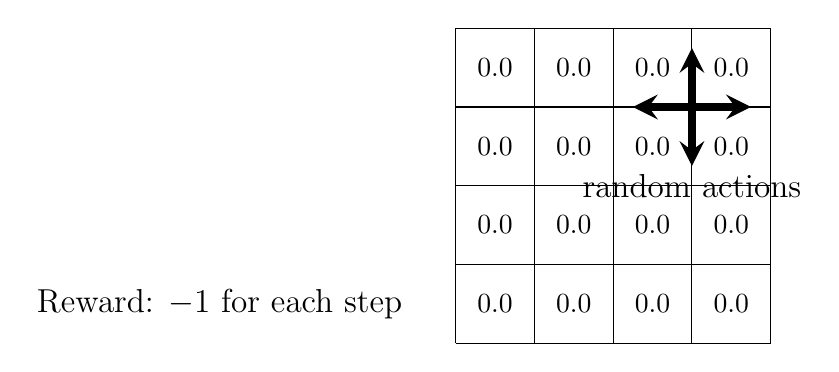
\begin{tikzpicture}
    \draw[stealth-stealth, line width=1 mm] (3.75, 3) -- (2.25, 3);
    \draw[stealth-stealth, line width=1 mm] (3, 2.25) -- (3, 3.75);
    \node at (3, 2) {\large random actions};
    \node at (-3, 0.5) {\large Reward: $-1$ for each step};
    % Top row.
    \node at (0.5, 3.5) {0.0};
    \node at (1.5, 3.5) {0.0};
    \node at (2.5, 3.5) {0.0};
    \node at (3.5, 3.5) {0.0};
    % Second frop top row.
    \node at (0.5, 2.5) {0.0};
    \node at (1.5, 2.5) {0.0};
    \node at (2.5, 2.5) {0.0};
    \node at (3.5, 2.5) {0.0};
    % Second from bottom row.
    \node at (0.5, 1.5) {0.0};
    \node at (1.5, 1.5) {0.0};
    \node at (2.5, 1.5) {0.0};
    \node at (3.5, 1.5) {0.0};
    % Bottom row.
    \node at (0.5, 0.5) {0.0};
    \node at (1.5, 0.5) {0.0};
    \node at (2.5, 0.5) {0.0};
    \node at (3.5, 0.5) {0.0};
    \draw[step=1.0,black] (0,0) grid (4, 4);
  \end{tikzpicture}
\end{document}